\section*{2.18}
From lecture we know that for an Einstein solid with $N$ atoms the multiplicity is
\eq{
\Omega(N,q) &= \cv{q+N-1 q}\\
&= (q+N-1)!/q!(N-1)!
}
Note that
\eq{
k! &= k(k-1)!
}
So the multiplicity becomes
\eq{
\Omega(N,q) &= N/q+N (q+N)!/q!N!
}
Strling's approximation says that
\eq{
N! & \approx sqrt{2\pi N}( N/e )^N
}
So we can substitute the equation above
\eq{
\Omega(N,q) & \approx N/q+N sqrt{ q+N/qN2\pi } ( q+N/e )^{q+N}( e/q )^q( e/N )^N\\
& \approx N/q+N sqrt{ q+N/qN2\pi } (q+N)^q( 1/q )^q(q+N)^N( 1/N )^N\\
& \approx N/q+N sqrt{ q+N/qN2\pi } ( q+N/q )^q( q+N/N )^N\\
& \approx \sqrt{ N/q(q+N)2\pi} ( q+N/q )^q( q+N/N )^N
}
\section*{3.25}
\subsection*{a}
The entropy is
\eq{
S = k_B\ln(\Omega(N,q))\\
& \approx k_B\ln(\sqrt{ N/q(q+N)2\pi} ( q+N/q )^q( q+N/N )^N)\\
& \approx k_B( 1/2 \ln( N/q(q+N)2\pi ) + \ln(( q+N/q )^q( q+N/N )^N))
}
The first term is of inferior order compared to the second term, so we feel free to neglect it, leading to the multiplicity provided
\eq{
S & \approx k_B \ln(( q+N/q )^q( q+N/N )^N)
}
\subsection*{b}
The chain rule gives us
\eq{
 1/T &= ppU0S \\
&= ppq0S ddU0q \\
&= \frac{k_B}{\epsilon} ppq0 \ln(( q+N/q )^q( q+N/N )^N)\\
&= \frac{k_B}{\epsilon} ppq0 ( q\ln( q+N/q ) + N\ln( q+N/N ))\\
&= \frac{k_B}{\epsilon} ppq0 ( q\ln(q+N) - q\ln(q) +N\ln( q+N/N ))\\
&= \frac{k_B}{\epsilon} (\ln(q+N) + q/q+N - \ln(q) -1 + N N/q+N 1/N )\\
&= \frac{k_B}{\epsilon} (\ln(q+N) - \ln(q))\\
&= \frac{k_B}{\epsilon} \ln( q+N/q )\\
\implies T &= \frac{\epsilon}{k_B} (\ln( q+N/q ))^{-1}
}
\subsection*{c}
Inverting the relationship in part b we get
\eq{
 1/T &= \frac{k_B}{\epsilon} \ln( q+N/q )\\
 \ex{ \frac{\epsilon}{Tk_B}} &= 1 + N/q \\
U &= \epsilon N (\ex{\frac{\epsilon}{Tk_B}}-1)^{-1}
}
Differentiating
\eq{
ppT0U &= \epsilon N ppT0 (\ex{\frac{\epsilon}{Tk_B}}-1)^{-1}\\
&= -\epsilon N (\ex{ \frac{\epsilon}{Tk_B}})^{-2} ppT0 \ex{\frac{\epsilon}{Tk_B}}\\
C &= \frac{1}{T^2} \frac{\epsilon^2 N}{k_B} \ex{\frac{\epsilon}{Tk_B}}(\ex{\frac{\epsilon}{Tk_B}}-1)^{-2}
}
\subsection*{d}
Taylor expanding the exponentials
\eq{
C &= \frac{\epsilon N}{T^2}\frac{\epsilon}{k_B}((\frac{Tk_B}{\epsilon})^2 + \frac{Tk_B}{\epsilon})\\
&= \epsilon N (\frac{k_B}{\epsilon}+\frac{1}{T})
}
Taking the limit $T \rightarrow \infty$
\eq{
C &= k_B N
}
\pagebreak
\subsection*{e}
This graph is most similar to lead. It differs from all three graphs in the low temperature limit, where it drops to $0$ too fast.
\begin{figure}[h]
    \centering
    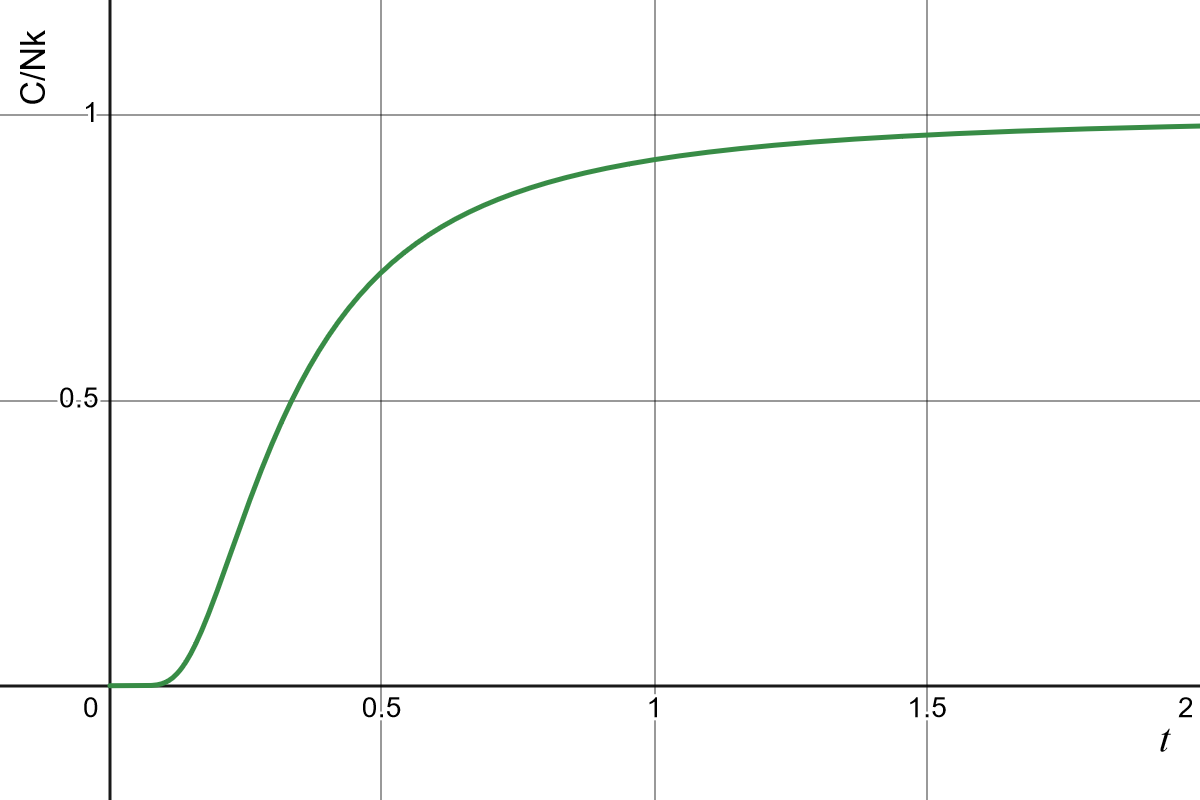
\includegraphics[width=1\linewidth]{Resources//112//Homework 2/112 Homework 2 Problem 2.png}
    \caption{Normalized Heat Capacity $\frac{C}{Nk_B}$ vs $\frac{k_BT}{\epsilon}$}
    \label{fig:enter-label}
\end{figure}

Start by writing down the heat capacity in terms of the high temperature limit $C(T_{high})$
\eq{
C &= \frac{1}{T^2} \frac{\epsilon^2 N}{k_B} \ex{\frac{\epsilon}{Tk_B}}(\ex{\frac{\epsilon}{Tk_B}}-1)^{-2}\\
&= (\frac{\epsilon}{Tk_B})^2C(T_{high}) \ex{\frac{\epsilon}{Tk_B}}(\ex{\frac{\epsilon}{Tk_B}}-1)^{-2}\\
C(\frac{\epsilon}{k_B}) &= C(T_{high})e(e-1)^{-2}\\
&\approx 0.92\cdot C(T_{high})
}
$C(T_{high})$ for lead, aluminum, and diamond are about $25$, $23$, and $12$, respectively. It follows that $C(\frac{\epsilon}{k_B})$ is $23$, $21$, and $11$. Which correspond to the temperatures (in Kelvin) $75$, $200$, and $400$. Multiplying by Boltzman's constant we can estimate $\epsilon$ (in eV) to be $0.00646eV$, $0.0172eV$, $0.0344eV$ for each material, respectively.
\subsection*{f}
Let $\chi = \frac{\epsilon}{k_B T}$, then
\eq{
C &= Nk_B \chi^2 \ex{\chi}(\ex{\chi}-1)^{-2}\\
}
Taylor expanding to third order
\eq{
C &= Nk_B \chi^2 (1+\chi+\frac{\chi^2}{2}+\frac{\chi^3}{6})(\chi+\frac{\chi^2}{2}+\frac{\chi^3}{6})^{-2}\\
}
We can immediately drop the $\chi^3$ terms\footnote{What was the point of expanding to 3rd order to drop 3rd order terms?} and distribute $\chi^2$
\eq{
C &= Nk_B((1+\frac{\chi}{2}+\frac{\chi^2}{6})^{-2}+\chi(1+\frac{\chi}{2}+\frac{\chi^2}{6})^{-1})\\
&= Nk_B((1+\chi+\frac{7\chi^2}{12})^{-1}+\chi(1+\frac{\chi}{2}+\frac{\chi^2}{6})^{-1})\\
}
We now Taylor expand $C(\chi)$ around $\chi \approx 0$, since we're neglecting higher order terms, it suffices to only compute the first three terms
\eq{
C(0) &= Nk_B\\
\frac{C'(\chi)}{Nk_B} &= -(1+\chi+\frac{7\chi^2}{12})^{-2}(1+\frac{7\chi}{6})^2+(1+\frac{\chi}{2}+\frac{\chi^2}{6})^{-1}\\
&-(1+\frac{\chi}{2}+\frac{\chi^2}{6})^{-2}(\frac{\chi}{2}+\frac{\chi^2}{3})\\
\frac{C'(0)}{Nk_B} &= -1 + 1 - 0 = 0\\
\frac{C''(\chi)}{Nk_B}&= 2(1+\chi+\frac{7\chi^2}{12})^{-3}(1+\frac{7\chi}{6})^2-\frac{7}{6}(1+\chi+\frac{7\chi^2}{12})^{-2}\\
&-(1+\frac{\chi}{2}+\frac{\chi^2}{6})^{-2}(\frac{1}{2}+\frac{\chi}{3})\\
&+2(1+\frac{\chi}{2}+\frac{\chi^2}{6})^{-3}(\frac{1}{2}+\frac{\chi}{3})^2\chi\\
&-(1+\frac{\chi}{2}+\frac{\chi^2}{6})^{-2}(\frac{1}{2}+\frac{2\chi}{3})\\
\frac{C''(0)}{Nk_B}&= 2-\frac{7}{6}-\frac{1}{2}-\frac{1}{2} = -\frac{2}{12}\\
\implies C(\chi) &\approx Nk_B - \frac{1}{2!}\frac{2}{12}\chi^2\\
&\approx Nk_B(1-\frac{1}{12}(\frac{\epsilon}{k_BT})^2)
}